As discussed in Sec.~\ref{sec:elastoplast}, plasticity is a property of solid materials, which is characterized by non-reversible deformations and plastic yielding of the material. The last mentioned material property can be mathematically described introducing so-called yield conditions $\Phi_{\mathrm{pl}}(\miu{\sigma}{}{})$. Fig. \ref{Mp_fig:yieldsfc} illustrates geometrically three typical yield conditions defined in the principal stress space. If the stress path of any material point is located inside of one of these surfaces, the point undergoes elastic deformation, if it is located on the boundary of the specific yield surface, plastic yielding is observed. The yield status of a material point is determined checking the Kuhn-Tucker conditions for loading or unloading:

\begin{equation}
{\dot{\Phi}}_{\mathrm{pl}} \leq 0, \qquad 
\lambda_{\mathrm{pl}}\,{\Phi_{\mathrm{pl}}}\,=\,0 \quad\mbox{or}\quad
\lambda_{\mathrm{pl}}\,\geq\,0
\label{Mp_kuhn_tucker}
\end{equation}

\begin{figure}[!htb]
  \begin{center}
   \begin{minipage}[t]{0.48\textwidth}
     \begin{center}
    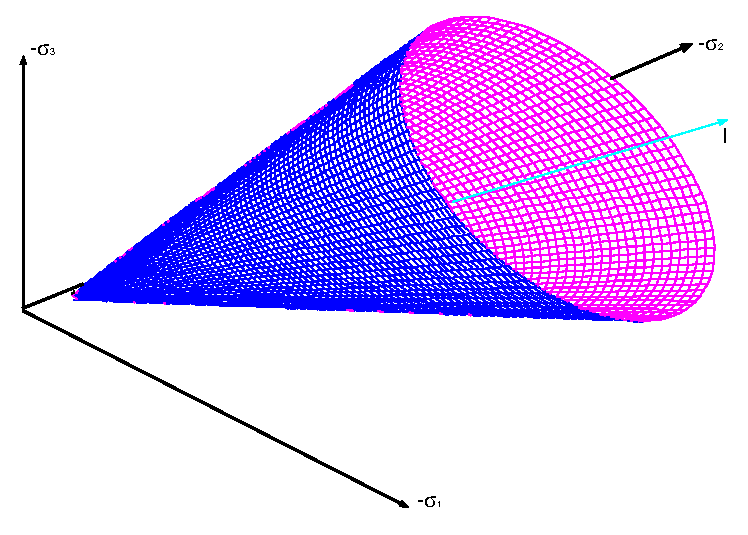
\includegraphics[scale=0.28]{PART_II/M/yieldsfc_dp.eps}
    \centerline{(Drucker-Prager)}
    \end{center}
   \end{minipage}
   \hspace{0.02\textwidth}
   \begin{minipage}[t]{0.48\textwidth}
    \begin{center}
    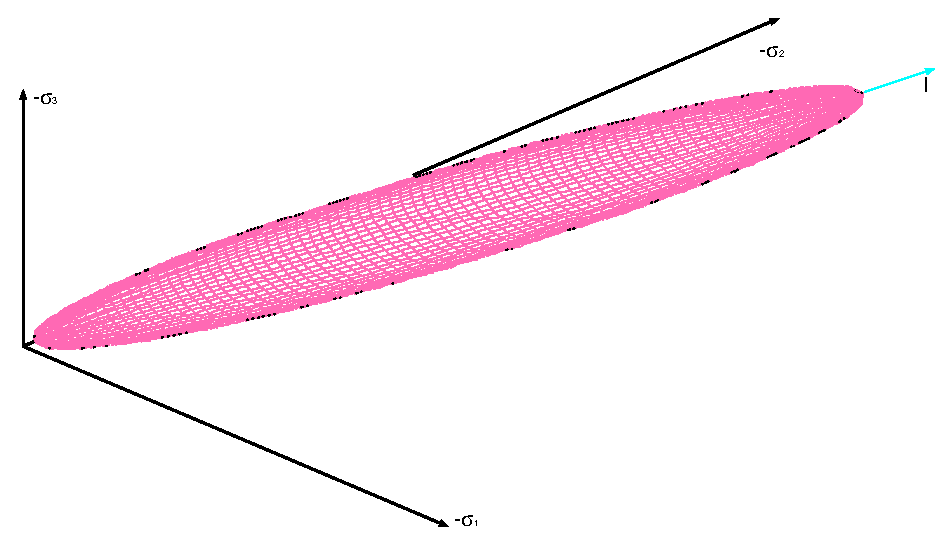
\includegraphics[scale=0.28]{PART_II/M/yieldsfc_cam.eps}\\
    \centerline{(Cam-Clay)}
    \end{center}
   \end{minipage}\\
   %
   \begin{minipage}[t]{0.48\textwidth}
     \begin{center}
    \includegraphics[scale=0.28]{PART_II/M/yieldsfc_wm.eps}
    \centerline{(Single yield surface)}
    \end{center}
   \end{minipage}
  \end{center}
  \caption{Yield surface}
  \label{Mp_fig:yieldsfc}
\end{figure}

In metal plasticity, usually so-called associative plasticity models are used, which are characterized by coaxiality of the plastic strain increment and the normal vector established in the current stress point of the yield condition. Usually, the mechanical behavior of geomaterials (in particular soils, and clay-rich materials) is of more complex nature compared to metals, and depends on porosity, stress state and direction of external loading. Frequently, shear deformation (shear bands) associated with strain localizytion, dilation and/or a coupling of these properties can be observed. Localization problems are of unstable nature, i.\,e., softening may occur at a certain point of loading. As these phenomena cannot be modeled using classical plasticity approaches, usually so-called non-associated plasticity models are introduced. They are characterized by the definition of a plastic potential ${\widehat{\Phi}}_{\mathrm{pl}}(\miu{\sigma}{}{})$ instead of the yield condition. Within this context, the increment of the plastic strain tensor will still be defined using Eq.~(\ref{eq:plaststrainrate}), but substituting the yield condition with the plastic potential. Two typical plastic models suited to address strain localization phenomena are described below.

\medskip
{\sl Drucker-Prager model}

This model is a function of two stress invariants and a hardening parameter $\kappa$ with the following yield condition and plastic potential:

\begin{eqnarray}
\Phi_{\mathrm{pl}}(\miu{\sigma}{}{},\kappa) & = &
\sqrt{\ttfrac{2}{3}\miu{\sigma}{d}{}\ccdot\miu{\sigma}{d}{}}\,+\,\alpha\,\mathrm{tr}(\miu{\sigma}{}{})\,-\,y(\kappa)\,=\,0 \\[1.0ex]
{\widehat{\Phi}}_{\mathrm{pl}}(\miu{\sigma}{}{},\kappa) & = &
\sqrt{\ttfrac{2}{3}\miu{\sigma}{d}{}\ccdot\miu{\sigma}{d}{}}\,+\,\beta\,\mathrm{tr}(\miu{\sigma}{}{})\,-\,y(\kappa)\,=\,0
\label{Mp_eqn:dp}
\end{eqnarray}
where $\alpha$ is a coefficient related to the internal frictional angle, $y(\kappa)$ is the yield stress depending on the hardening parameter.


\medskip
{\sl Cam-Clay model}

Similar to the Drucker-Prager model, the Cam-Clay model is a funtion of both of the first and the second stress invariants. The generalized Cam-Clay model is defined as:

\begin{eqnarray}
\Phi_{\mathrm{pl}}(\miu{\sigma}{}{},\kappa)\,=\,
\ttfrac{2}{3}\miu{\sigma}{d}{}\ccdot\miu{\sigma}{d}{}\,+\,M^2\,p_s\,(p_s-{p_s}_{cn})\,=\,0
\label{Mp_eqn:cc}
\end{eqnarray}
with $p_s=\mathrm{tr}(\miu{\sigma}{}{})/3$, where $M$ is the slope of the critical state line and ${p_s}_{cn}$ is the isotropic preconsolidation pressure. The rate of $p_s$ is given by

\begin{equation}
\frac{\mathrm d\, p_s}{\mathrm d\,\varepsilon^{\mathrm v}_{\mathrm{pl}}}\,=\,
\frac{(1+e)p_s}{\lambda_c-\kappa_c}
\label{Mp_eqn:cc_pcn}
\end{equation}
where $e$ is the void ratio, $\varepsilon^{\mathrm v}_{\mathrm{pl}}$ defines the volumetric plastic strain, $\lambda_c$ is the virgin compression index and $\kappa_c$ is the swelling/recompression index.

The model also describes the nonlinear elastic behavior of clay-like media before plastic yielding occurs, in which the bulk modulus $K$ is dependent of stress status as

\begin{eqnarray}
K=\frac{1+e}{\kappa_c}p_s=0
\label{Mp_eqn:cc_K}
\end{eqnarray}
